\documentclass[tikz,border=2pt]{standalone}
\pdfmapfile{+cm.map}
\usepackage{pgfplots}
\pgfplotsset{compat=1.18}
\usetikzlibrary{arrows.meta}
\definecolor{ink}{HTML}{202B30}
\definecolor{red}{HTML}{971D2C}
\definecolor{soft}{HTML}{F4E9EB}
\definecolor{gray}{HTML}{51636D}
\definecolor{line}{HTML}{D6DDE0}
\definecolor{pale}{HTML}{F0F3F4}
\begin{document}
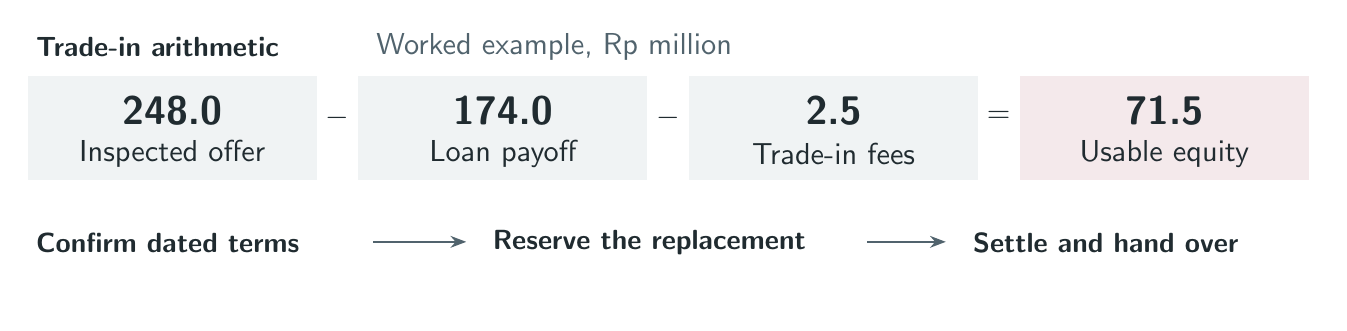
\begin{tikzpicture}[x=1cm,y=1cm,font=\sffamily\fontsize{10.5}{12}\selectfont,text=ink,arr/.style={-{Stealth[length=2mm]},draw=gray,thick}]
\path[use as bounding box] (0,0) rectangle (16.4,3.5);
\node[anchor=west,inner sep=0pt,font=\sffamily\bfseries] at (0.1,3.25) {Trade-in arithmetic};
\node[anchor=west,inner sep=0pt,text=gray] at (4.42,3.25) {Worked example, Rp million};
\fill[pale] (0,1.56) rectangle (3.67,2.89);
\node[align=center,inner sep=0pt,font=\sffamily\Large\bfseries] at (1.835,2.44) {248.0};
\node[align=center,inner sep=0pt,] at (1.835,1.9) {Inspected offer};
\fill[pale] (4.2,1.56) rectangle (7.87,2.89);
\node[align=center,inner sep=0pt,font=\sffamily\Large\bfseries] at (6.035,2.44) {174.0};
\node[align=center,inner sep=0pt,] at (6.035,1.9) {Loan payoff};
\fill[pale] (8.4,1.56) rectangle (12.07,2.89);
\node[align=center,inner sep=0pt,font=\sffamily\Large\bfseries] at (10.235,2.44) {2.5};
\node[align=center,inner sep=0pt,] at (10.235,1.9) {Trade-in fees};
\fill[soft] (12.6,1.56) rectangle (16.27,2.89);
\node[align=center,inner sep=0pt,font=\sffamily\Large\bfseries] at (14.434999999999999,2.44) {71.5};
\node[align=center,inner sep=0pt,] at (14.434999999999999,1.9) {Usable equity};
\node[align=center,inner sep=0pt,] at (3.93,2.36) {$-$};
\node[align=center,inner sep=0pt,] at (8.13,2.36) {$-$};
\node[align=center,inner sep=0pt,] at (12.33,2.36) {$=$};
\node[anchor=west,inner sep=0pt,font=\sffamily\bfseries] at (0.1,0.77) {Confirm dated terms};
\node[anchor=west,inner sep=0pt,font=\sffamily\bfseries] at (5.9,0.77) {Reserve the replacement};
\node[anchor=west,inner sep=0pt,font=\sffamily\bfseries] at (12,0.77) {Settle and hand over};
\draw[arr] (4.39,0.78) -- (5.57,0.78);
\draw[arr] (10.66,0.78) -- (11.66,0.78);
\end{tikzpicture}\end{document}